\documentclass{beamer}
\usepackage[utf8]{inputenc}
\usepackage{graphicx, epsfig}
\usepackage{amsmath,mathrsfs,amsfonts,amssymb}
\usepackage{subfig}
\usepackage{floatflt}
\usepackage{epic,ecltree}
\usepackage{mathtext}
\usepackage{fancybox}
\usepackage{fancyhdr}
\usepackage{multirow}
\usepackage{enumerate}
\usepackage{epstopdf}
\usepackage{multicol}
\usetheme{Copenhagen}%{Singapore}%{Warsaw}%{Warsaw}%{Darmstadt}
\usecolortheme{whale}
%\definecolor{beamer@blendedblue}{RGB}{15,120,80}

\newcommand{\T}{{\text{\tiny\sffamily\upshape\mdseries T}}}
%--------------------------------------------------------------------------------
\title[\hbox to 56mm{Human Activity Recognition  \hfill\insertframenumber\,/\,\inserttotalframenumber}]
{Generative models for human activity recognition}
\author[ROY team]{\\
				{\small \textbf{ROY team:} Ilya Zharikov, Roman Isachenko, \\
					Artem Bochkarev}}
\institute[SkolTech]{Skolkovo Institute of Science and Technology \\
	Machine Learning course 
    \vspace{0.3cm}
}
\date{March 20, 2017.}
%--------------------------------------------------------------------------------
\begin{document}
%--------------------------------------------------------------------------------
\begin{frame}
%\thispagestyle{empty}
\titlepage
\end{frame}
%--------------------------------------------------------------------------------
\begin{frame}{Project goal}
	
	\begin{block}{Aim}
		Classification model for complex-structured objects.
	\end{block}

	\begin{block}{Problem}
		Initial object has no appropriate feature description.
	\end{block}
	
	\textbf{Applications:}
	\begin{itemize}
		\item image processing;
		\item signal classification;
		\item topic modelling;
		\item \textit{time series analysis}.
	\end{itemize}
	
\end{frame}
%--------------------------------------------------------------------------------
\begin{frame}{Related work}
	\begin{enumerate}
		\item Wang W. et al. Human activity recognition using smart phone embedded sensors // \emph{International Joint Conference on Neural Networks}. 2014.
		\item Kwapisz, Jennifer R., Gary M. Weiss, and Samuel A. Moore. Activity recognition using cell phone accelerometers. // \emph{ACM SigKDD Explorations Newsletter}. 12(2): 74-82. 2011.
		\item Kuznetsov M. P., and Ivkin N. P. Time series classification algorithm using combined feature description. // \emph{Journal of Machine Learning and Data Analysis}. 2015.
	\end{enumerate}
	
\end{frame}
%--------------------------------------------------------------------------------
%\section{Problem Statement}
\begin{frame}{Problem Statement}
	\begin{itemize}
		\item $s \in \mathcal{S}$ - complex structured object
		\item $y \in Y$ - class label
	\end{itemize}
	\begin{block}{Task}
	Given: $\mathfrak{D} = \{(s_i, y_i)\}_{i=1}^m$ recover
	\[
		y = f(s) \quad \forall s \in \mathcal{S}.
	\]
	\end{block}
	\begin{block}{Approach}
		Suppose $f = g \circ h$, where
		\begin{itemize}
			\item $h(s): \mathcal{S} \rightarrow H \in \mathbb{R}^n$,  $\mathbf{h}_i = h(s_i)$;
			\item $g(\mathbf{h}, \theta)$~--- parametric map from $H$ into $Y$ (classification model).
		\end{itemize}
	\end{block}
\end{frame}
%--------------------------------------------------------------------------------
\begin{frame}{Optimal parameters}
	\begin{enumerate}
		\item Choice of feature map $h(s)$ by 
		\begin{itemize}
			\item prior (expert) knowledge;
			\item minimizing error functional.
		\end{itemize}
		
		\item Classification for $\{(\mathbf{h}_i , y_i)\}_{i=1}^m$
		\[
			\mathbb{\theta}^* = \arg \min_{\theta} L(g, \theta, \mathfrak{D}).
		\]
		E.g. 
			$g(\mathbf{h}, \theta)$ - classification model, \\ \hspace{0.7cm}
			$\theta$ - model parameters, \\ \hspace{0.7cm}
			$L (g, \theta, \mathfrak{D})$ - classification error function.
		
	\end{enumerate}

\end{frame}
%--------------------------------------------------------------------------------
\begin{frame}{Time series example}
	\begin{figure}[h]
		\centering
		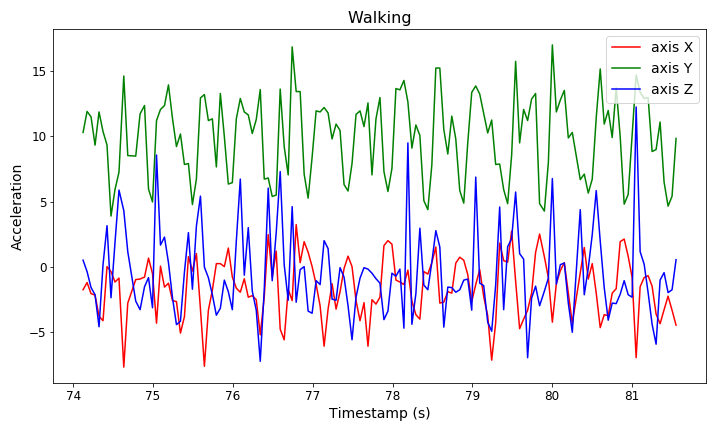
\includegraphics[width=1\linewidth]{ts_example.png}
		\label{ts_example}
	\end{figure}
\end{frame}
%--------------------------------------------------------------------------------
%\section{Feature extraction}
\begin{frame}{Expert functions}
	Prior knowledge about the objects could allow to choose the features.
	\begin{block}{Feature description}
		$\mathbf{h}_i = h(s_i)\in \mathbb{R}^{40}$~--- different statistics:
		\begin{itemize}
			\item average acceleration;
			\item standard deviation;
			\item mean absolute deviation;
			\item ...
		\end{itemize}
	\end{block}

\end{frame}
%--------------------------------------------------------------------------------
\begin{frame}{Autoregressive model}
	\begin{block}{Data generation hypothesis}
		Time series $s = (x_1, \dots, x_T)$ is generated by autoregressive model
		\[
			\hat{x}_t = w_0 + \sum_{j=1}^n w_j x_{t-j}.
		\]
	\end{block}
	
	\begin{block}{Feature description}
		\[
			h(s_i) = \mathbf{w}^* = \arg \min_{\mathbf{w} \in \mathbb{R}^{n+1}} \sum_{j=n+1}^{T} \| x_j - \hat{x}_j \|^2.
		\]
	\end{block}
\end{frame}
%--------------------------------------------------------------------------------
\begin{frame}{Singular Spectrum Analysis (SSA)}
	Trajectory matrix for time series $s = (x_1, \dots, x_T)$:
	\[
		\mathbf{X} = 
		\begin{pmatrix}
			x_1 & x_2 & \dots & x_n \\
			x_2 & x_3 & \dots & x_{n+1} \\
			\dots & \dots & \dots & \dots\\
			x_{T-n+1} & x_{T-n+2} & \dots & x_{T}
		\end{pmatrix}.
	\]
	
	\begin{block}{Feature description}
		\[
			h(s_i) = (\lambda_1, \dots ,\lambda_n),
		\]
		where $\{\lambda_i\}_{i=1}^n$ are eigenvalues of the matrix $\mathbf{X}^{\T} \mathbf{X}$, obtained by SVD decomposition
		\[
			\mathbf{X}^{\T} \mathbf{X} = \mathbf{V} \cdot \text{diag} (\lambda_1, \dots, \lambda_n) \cdot \mathbf{V}^{\T}.
		\]
	\end{block}

\end{frame}
%--------------------------------------------------------------------------------
\begin{frame}{(?!) Splines}

\end{frame}
%--------------------------------------------------------------------------------
\begin{frame}{Data}
\noindent
\begin{minipage}[t]{0.45\linewidth}
	\textbf{WISDM}$^1$
	\begin{table}[]
		\small
		\label{my-label}
		\begin{tabular}{|l|c|}
			\hline
			Activity   & \# objects \\
			\hline
			Standing   & 229(5.3\%)  \\
			Walking    & 1917(44.4\%) \\
			Upstairs   & 466(10.8\%) \\
			Sitting    & 277(6.4\%)  \\
			Jogging    & 1075(24.9\%) \\
			Downstairs & 357(8.3\%) \\
			\hline
			Total & 4321  \\
			\hline
		\end{tabular}
	\end{table}

	\vspace{1cm}
	\medskip\hrule\medskip
	{\footnotesize $^1$http://www.cis.fordham.edu/wisdm/ \\
		$^2$http://sipi.usc.edu/HAD/}
	
\end{minipage}
\hfill
\begin{minipage}[t]{0.48\linewidth}
	\textbf{USC-HAD}$^2$
	\begin{table}[]
		\small
		\label{my-label}
		\begin{tabular}{|l|c|}
			\hline
			Activity & \# objects \\ \hline
			Standing           & 1167(8.6\%)  \\
			Elevator-up        & 764(5.6\%)  \\
			Walking-forward    & 1874(13.8\%) \\
			Sitting            & 1294(9.5\%)  \\
			Walking-down & 951(7\%)  \\
			Sleeping           & 1860(13.7\%) \\
			Elevator-down        & 763(5.6\%)  \\
			Walking-upstairs        & 1018(7.4\%)  \\
			Jumping        & 495(3.6\%)  \\
			Walking-right        & 1305(9.6\%)  \\
			Walking-left        & 1280(9.4\%)  \\
			Running            & 849(6.2\%)  \\ \hline 
			Total              & 13620                                \\ \hline
		\end{tabular}
	\end{table}
\end{minipage}

\end{frame}
%--------------------------------------------------------------------------------
\begin{frame}{Experiment}
	\begin{itemize}
		\item datasets: WISDM, USC-HAD;
		\item feature extraction methods: expert functions, autoregressive models, singular spectral analysis, splines;
		\item classification models: logistic regression, support vector machine, random forest;
		\item tuning parameters: cross-validation;
		\item quality measure: accuracy score.
	\end{itemize}

\end{frame}
%--------------------------------------------------------------------------------
\begin{frame}{Results}
	\begin{table}[]
		\centering
		\label{my-label}
		\begin{tabular}{|l|c|c|c|c|}
			\hline
			 & Expert & AutoReg & SSA & Splines\\
			\hline
			Log-Reg &    0.668    &    0.651     &   0.637  & 0.415  \\
			\hline
			SVM     &    0.797    &     0.655    &   0.822  & 0.740\\
			\hline
			RF      &    0.871    &     0.703    &  0.840 & 0.736 \\
			\hline
		\end{tabular}
	\end{table}

\end{frame}
%--------------------------------------------------------------------------------
\begin{frame}{Feature union}

\end{frame}
%--------------------------------------------------------------------------------
\begin{frame}{Conclusion}
	\begin{block}{Done}
		\begin{itemize}
			\item different approaches to classification of complex-structured objects were studied
			\item the results of experiments on human activities datasets outperform many previous methods
			\item 
		\end{itemize}
	\end{block}
	\begin{block}{Future work}
		\begin{itemize}
			\item new approaches to feature extraction (e.g. modified splines)
			\item implementing of structured learning methods
		\end{itemize}
	
	\end{block}
\end{frame}


\end{document} 